\section{Main result and mathematical context}\label{sec:intro}

\subsection{A concrete phenomenon}
Fix a finite field $\F_q$, an integer $n\ge1$, a nondegenerate alternating bilinear form on
$V=\F_q^{2n}$, and a finite simple graph $G$. At each vertex $v$, independently
choose a uniform nonzero vector $X_v$. An oriented edge $u\to v$ reveals
\[
Y_{uv}=\pair{X_u}{X_v}.
\]
Repeated vectors at different vertices are allowed. We compare these observations
with independent field elements having exactly the same one-edge distribution.

A tree reveals no dependence at all, regardless of its size. A cycle reveals
dependence only when all of its edges are retained: the joint law of any proper
subset of its edges is exactly the independent law. Nevertheless, enough complete
cycles permit nearly certain detection of the hidden common geometry. The number
required grows exponentially in the ambient dimension, and adding one edge to an
odd cycle does not change its leading information.

These statements concern the entire labelled edge vector. They are stronger than
a count of configurations with one specified label. The comparison retains
the true one-edge bias. Comparing instead with independent uniform labels would
introduce an additional signal already visible on single edges.

\begin{figure}[htbp]
\centering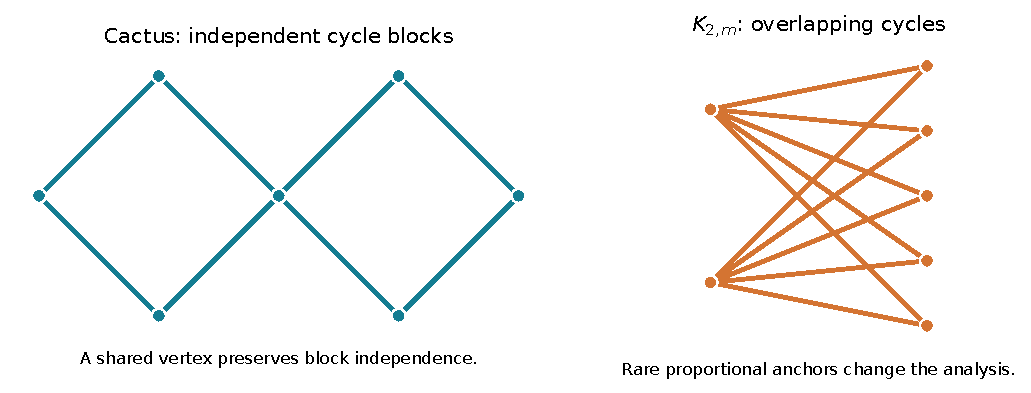
\includegraphics[width=.96\linewidth]{figures/observation_graphs.pdf}
\caption{Two observation patterns. Cycle blocks in a cactus are independent even when they share a vertex. Complete bipartite observations have overlapping cycles and a different detection calculation.}
\end{figure}

\subsection{The sharp detection theorem}
Put $N=q^{2n}$. For $\ell\ge3$ define
\begin{equation}\label{eq:info}
v_{\ell,N}=
\begin{cases}
\displaystyle (q-1)^\ell\frac{N}{(N-q)^\ell},&\ell\text{ odd},\\[7pt]
\displaystyle (q-1)^{\ell-2}
\bigl((N-q)^{2-\ell}+(q-2)(N-1)^{2-\ell}\bigr),&\ell\text{ even}.
\end{cases}
\end{equation}
A \emph{cactus} is a finite simple graph in which two distinct simple cycles
have at most one common vertex. Trees, disjoint unions of cycles, and arbitrarily
many cycles attached at one common vertex are examples.

\begin{theorem}[Sharp detection on growing cactus graphs]\label{thm:main}
Fix $q$ and an integer $L\ge3$. For each $n$, let $G_n$ be any cactus graph whose
cycle lengths belong to $\{3,\ldots,L\}$. The graph may have arbitrarily many
vertices and bridges. Let $P_n$ be its symplectic edge law and $Q_n$ the product
of its true one-edge marginals. Let $\mathcal C_n$ be its set of cycles and put
\[
I_n=\sum_{C\in\mathcal C_n}v_{|C|,q^{2n}}.
\]
Then:
\begin{enumerate}[label=(\roman*)]
\item If $I_n\to\tau\in[0,\infty)$, then
\begin{equation}\label{eq:profile}
\TV(P_n,Q_n)\longrightarrow 2\Phi(\sqrt{\tau}/2)-1,
\end{equation}
where $\Phi$ is the standard normal distribution function.
\item If $I_n\to\infty$, then $\TV(P_n,Q_n)\to1$.
\item If $0<\tau<\infty$, the log likelihood ratio converges in distribution to
$\mathcal N(-\tau/2,\tau)$ under $Q_n$ and to
$\mathcal N(\tau/2,\tau)$ under $P_n$. The minimum average error with equal prior
probabilities tends to $\Phi(-\sqrt{\tau}/2)$.
\end{enumerate}
All assertions include characteristic two.
\end{theorem}

For either of the two lengths $\ell=2r+1$ and $\ell=2r+2$,
\begin{equation}\label{eq:pair}
v_{\ell,N}=(q-1)^{2r+1}N^{-2r}(1+O_{q,r}(N^{-1})).
\end{equation}
Consequently, if a cactus has $m_n$ cycles, all of either one of these lengths
or any mixture of the two, its critical scale is
\begin{equation}\label{eq:critical}
m_n\asymp\frac{q^{4nr}}{(q-1)^{2r+1}}.
\end{equation}
More precisely, $m_n(q-1)^{2r+1}q^{-4nr}\to\tau$ gives
\eqref{eq:profile}. This is an equality of leading statistical information;
the two finite-dimensional laws need not coincide.

\subsection{What is inherited and what is added}
The supplied repository was inspected at commit
\texttt{00cadb961bbe77c74e5d082c4948f8884d58a970}.
Its merged article contains finite-field Fourier estimates, positive-type
stabilizer bounds, exact laws for two arbitrary symplectic frames, and numerous
rank and residual-form comparisons \cite{ProveItSpn}. In particular,
\texttt{spn:lem:alt-gram} evaluates Fourier coefficients of a random alternating
Gram matrix by the rank of the Fourier variable. The transfer from the original
proof program to finite-field statistics is also described in its source
section \cite{ProveItSrc}.

Several apparently natural extensions are already covered by current Research
packets: fixed-gap rectangular blocks, exact two-frame tests, and joint
rank/defect expansions \cite{ProveItTwo,ProveItRect}. We do not claim these.
Earlier work in the same research program also supplied a several-frame
threshold and forest independence. We take the forest observation as a starting
point and prove it again for self-containment.

The additions here are the full labelled cycle laws, their exact information and
distance formulas, the even-cycle resonance, the equality \eqref{eq:pair}, the
sharp growing-cactus testing theorem, and a contrasting overlapping-cycle family.
Classical symplectic graph spectra and finite-field cycle counts are adjacent
subjects \cite{TangWan,IJM,Bright}; individual fixed-label counts and the Fourier
technique alone are not presented as new. The broader question of
observation-graph-dependent detectability also has an established counterpart
for real Wishart models \cite{BBH}. Our statements specify an exact finite-field
experiment and its explicit critical profile. The novelty assessment is scoped
in \cref{sec:provenance}.

